\begin{figure}[t]

\rkc{Move all this code into the mockup screenshots below.}

\lstset{basicstyle=\scriptsize\ttfamily}
\begin{lstlisting}
type student_data =
  { name: string, hw1: float, hw2: float, hw3: float, midterm: float, final: float };

let grades : list(student_data) =
  [ { name: "Alice", hw1: 76.0, hw2: 93.0, hw3: 91.0, midterm: 77.0, final: 95.0 }
  , { name: "Bob"  , hw1: 88.0, hw2: 75.0, hw3: 80.0, midterm: 89.0, final: 87.0 }
  , ...
  ];

let weighted_average(g: student_data) =
  ??_a;          =====>        (10.0 *. g.hw1) +. ??_b;

let weighted_averages = List.map weighted_average grades;
\end{lstlisting}
%% restore settings from main.tex
\lstset{basicstyle=\footnotesize\ttfamily}

%% TODO once the code above is removed, scale up the screenshots
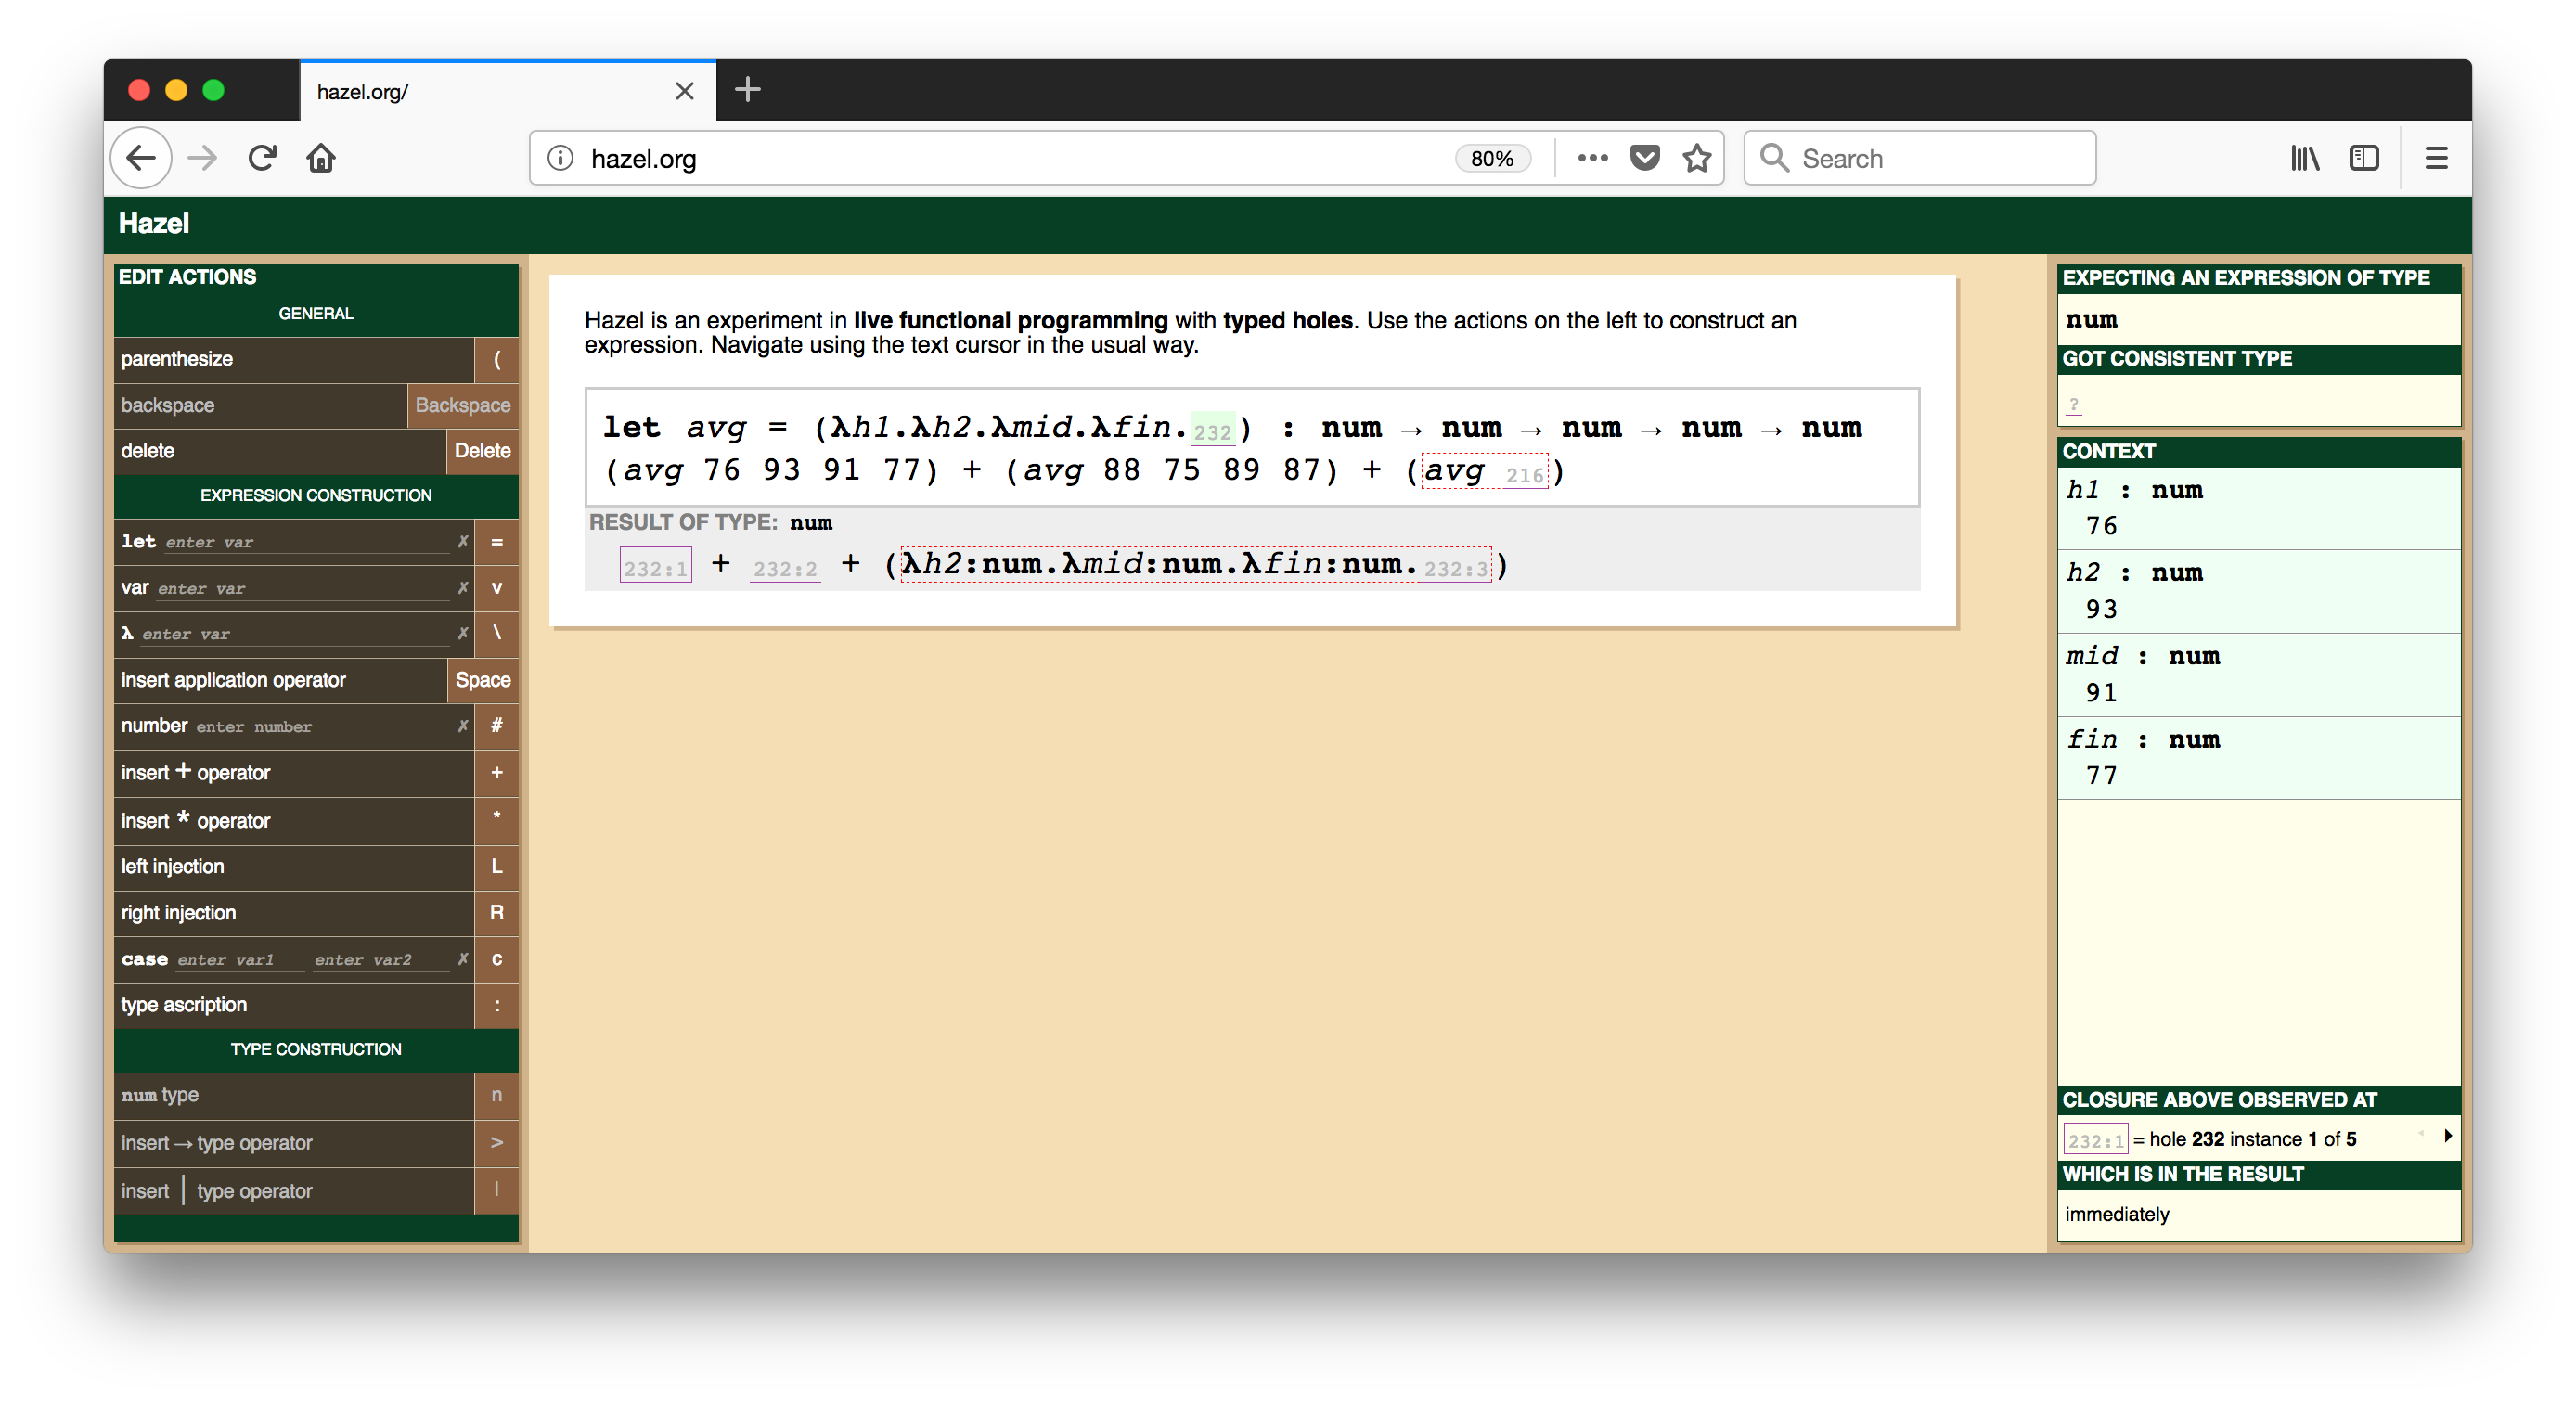
\includegraphics[scale=0.20]{images/hazel-placeholder-0.png}

\rkc{Draw arrows and captions on the top figure to show how to get
to the bottom figure.
ser navigates to hole a, types + to create a plus, types * to create a
multiplication, types \#10 to create 10, types vh1 to create variable use.}

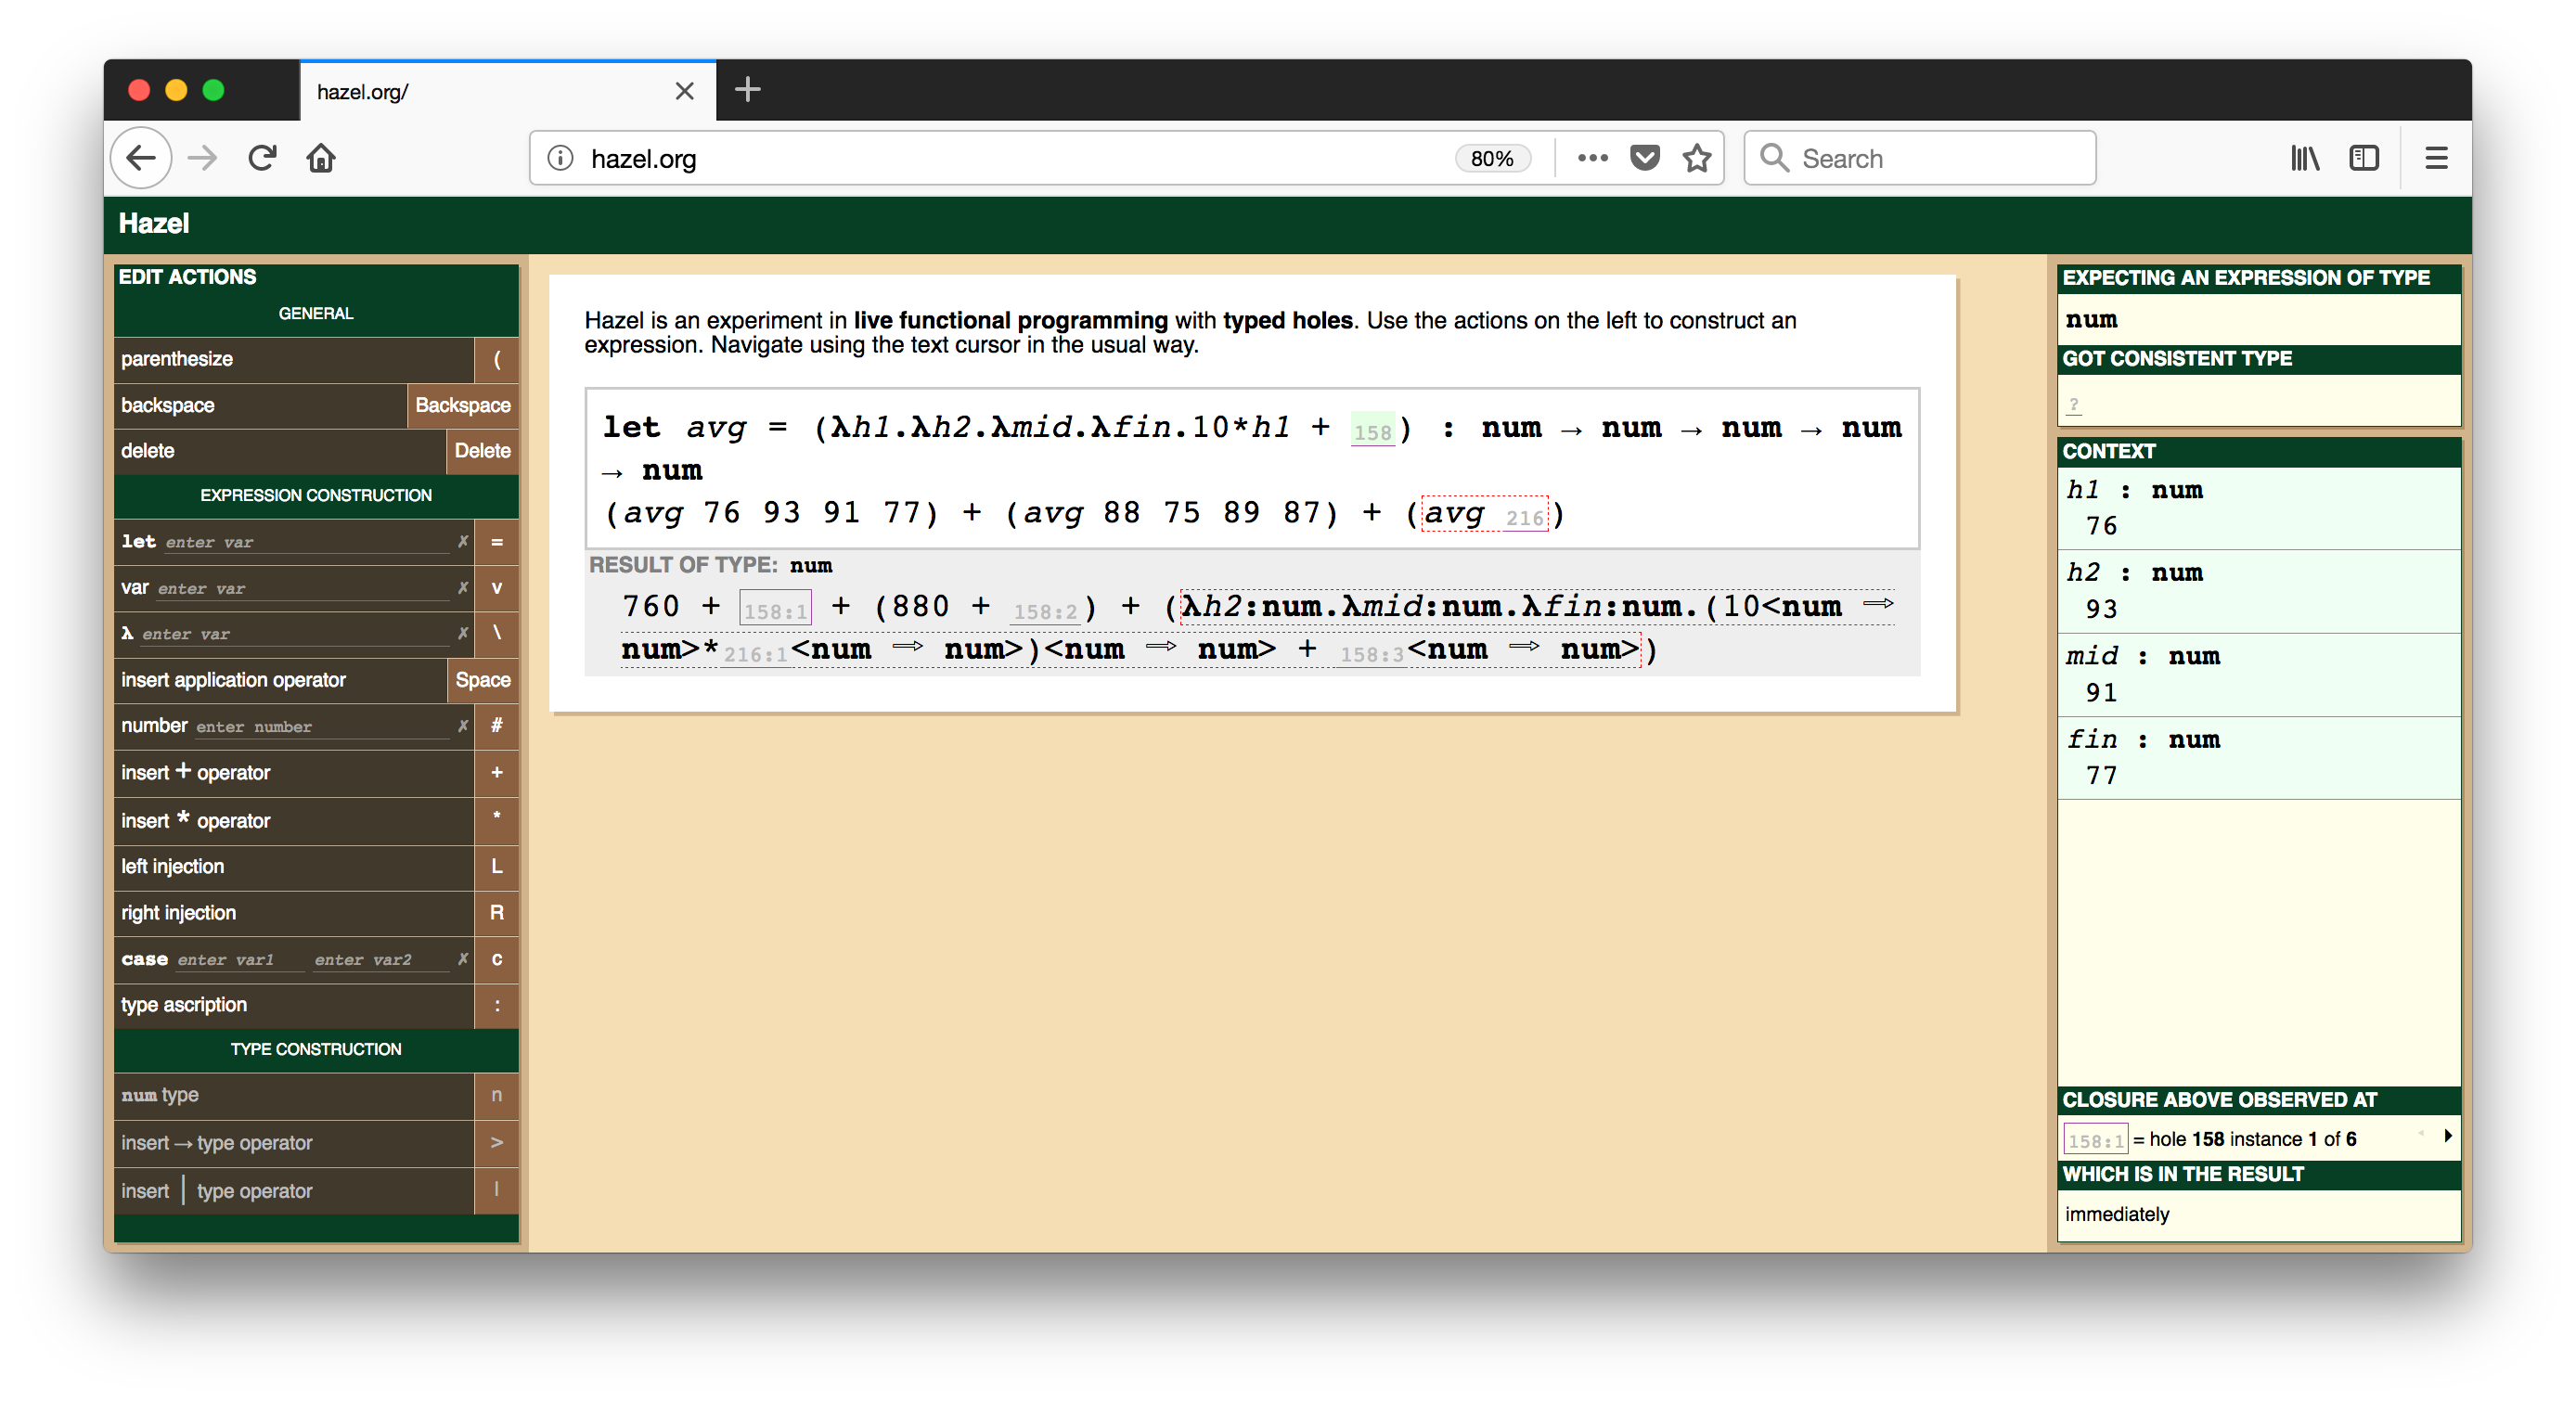
\includegraphics[scale=0.20]{images/hazel-placeholder-1a.png}

\caption{Hazel mockups for Example 1a.}
\label{fig:grades-example}
\end{figure}
